\subsection{All Predictions Summary View}
\label{sec:allPairs}
Since we can only focus on one individual example at a time for detail analysis,
how to pick an single pair of sentence from the development or test dataset (for the SNLI dataset, each of the these set consists of close to $10k$ examples) is an obvious challenge.
%
In addition, we also want to obtain certain high-level understand of how the whole set behave, beyond the information the prediction accuracy provide.

\begin{figure}[htbp]
\centering
\vspace{-2mm}
 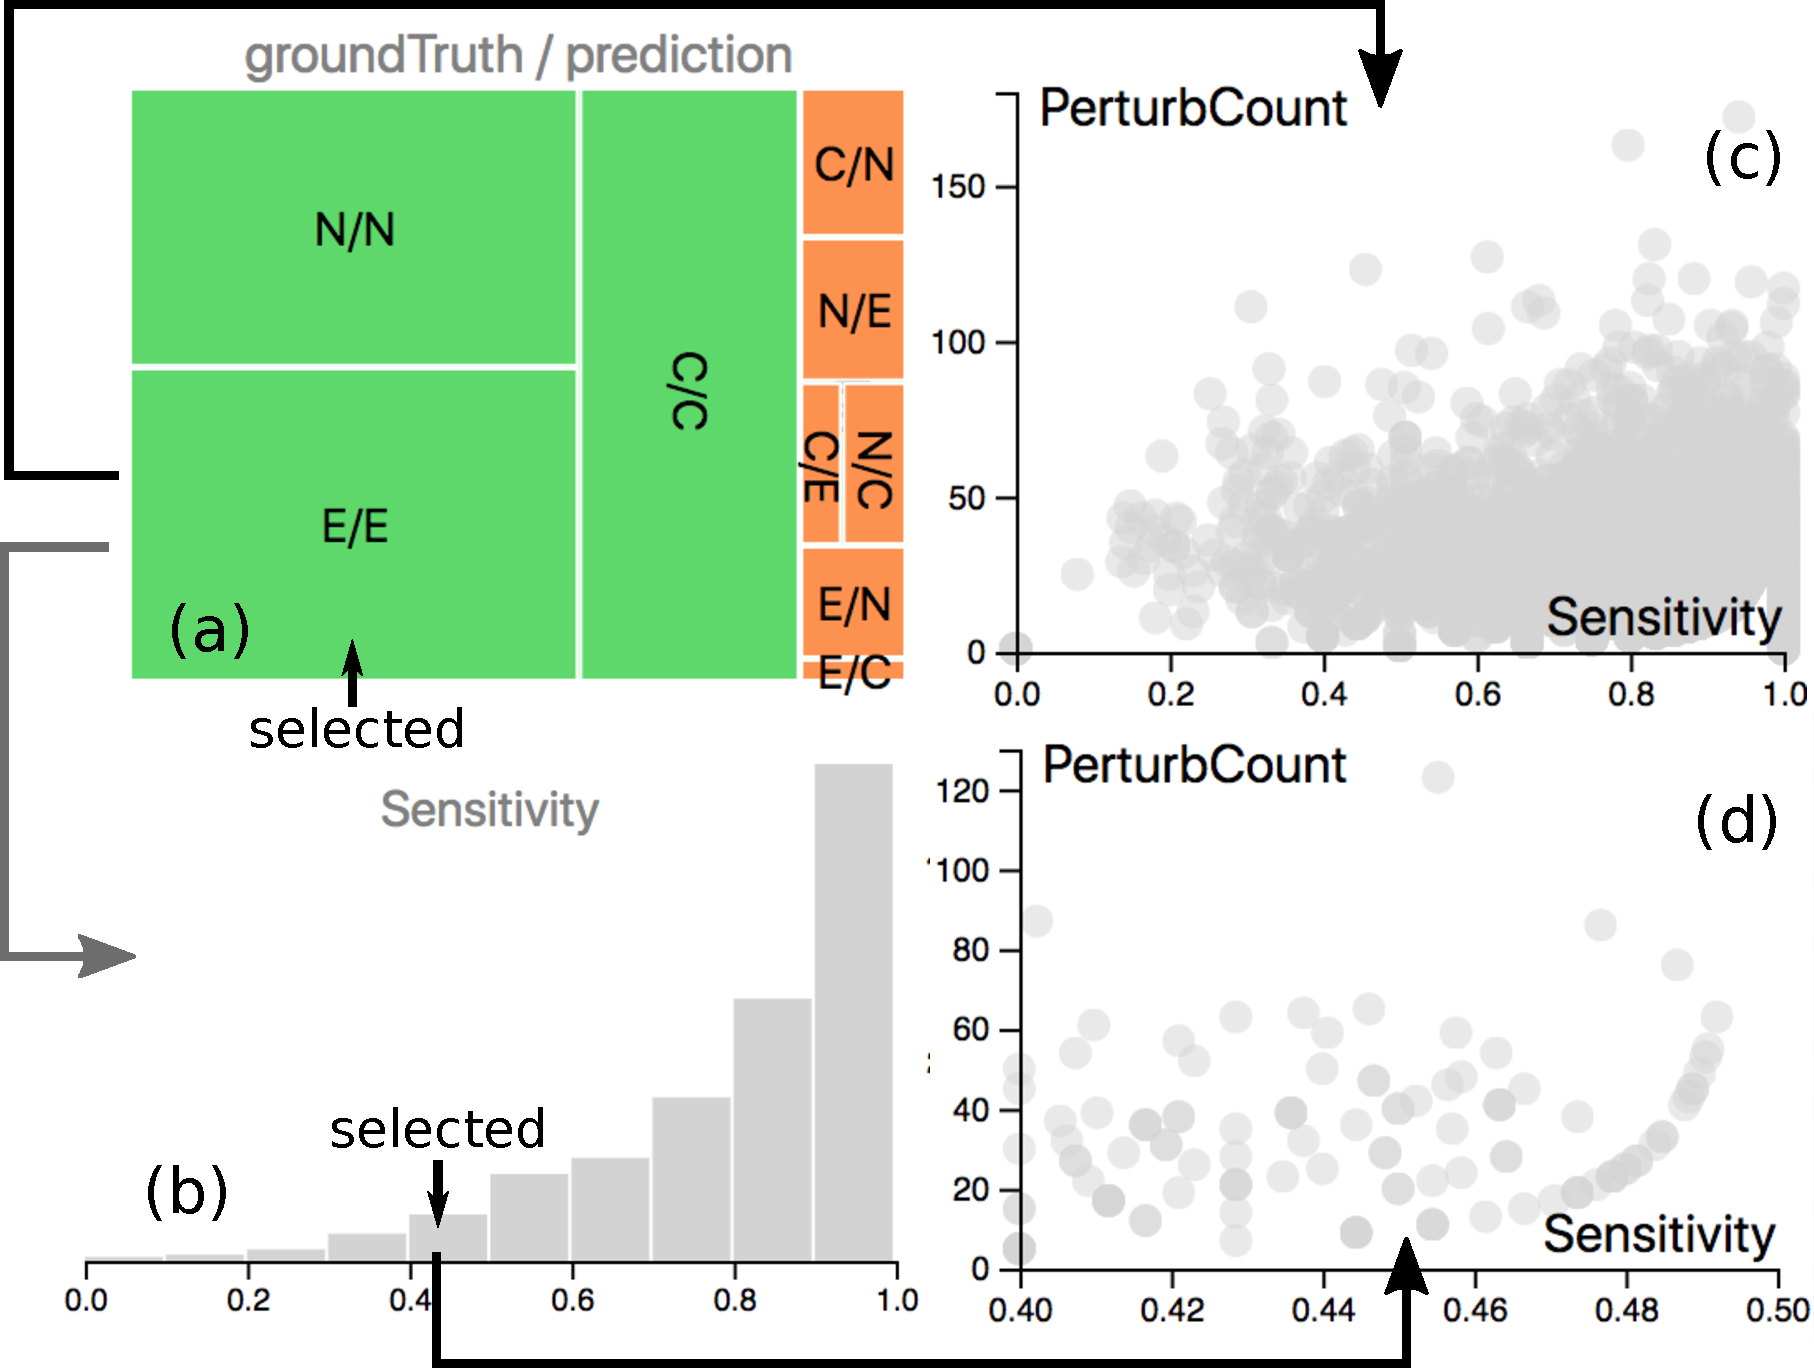
\includegraphics[width=1.0\linewidth]{summaryView}
 \caption{Explore the full development set and examine their prediction result and sensitivity.}
\label{fig:modelPipeline}
\end{figure}

%The all pair
\begin{itemize}
\item How to go from 10k pair to one pair
\item What constitute interesting example
\item How to get a sense of overall prediction result
\end{itemize}
